
\documentclass[a4paper]{article}

\usepackage[T1]{fontenc}
\usepackage[english]{babel}
\usepackage[utf8]{inputenc}
\usepackage{graphicx}
\usepackage{fancyhdr}
\usepackage{subcaption}
\usepackage{float}
\usepackage{tikz}
\captionsetup{margin=10pt,font=small,labelfont=bf}


\newcommand{\progname}{Cubic Steric Overlap Detector}
\newcommand{\doctitle}{Implementation details}


\pagestyle{fancy}
\topmargin -20.0pt
\headheight 56.0pt
\rhead{
  \progname\\
  \doctitle
}
\setlength{\topskip}{0pt} % Skip some whitespace at the top
\newcommand{\horrule}[1]{\rule{\linewidth}{#1}} % Create horizontal rule command with 1 argument of height


\begin{document}
\thispagestyle{plain} % No header for first page


\begin{center}
\horrule{0.5pt} \\[0.3cm] % Thin top horizontal rule
%
\huge  \progname \\[1mm]
\Large \doctitle
\normalsize % Revert to normal sized font

\horrule{2pt} \\[0.1cm] % Thick bottom horizontal rule

\begin{tabular}{ l r }
  By Johan Sjöblom & sjoblomj88@gmail.com
\end{tabular}\\[0.1cm]
\footnotesize Document version: 1.0, June 2014\\[0.4cm]

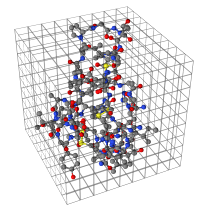
\includegraphics{res/molspace.png}
\end{center}
\horrule{0.5pt} % Thin top horizontal rule
\normalsize % Revert to normal sized font



\section*{Background and motivation}
When modelling proteins, or when docking a pair of proteins together, one might want to test whether the solution is free from steric clashes. That is, when considering atoms to be hard spheres, one wants to know whether any atoms are so close together that the spheres representing the atoms intersect in 3-D. This program will detect any such steric overlaps between two proteins read from Protein Data Bank files (*.pdb files). Proteins are complicated 3-D structures, and are often ``folded'' in such ways that it would be very complicated to predict whether an arbitrary atom is close to another in the molecule.

\subsection*{Constraints}
The problem is from an assignment given by my professor. A few constraints applied to the problem. All atoms could be assumed to have a radius of \mbox{2.0 Å}. The task was to minimise the number of atom-atom comparisons. Any pre-processing was allowed, and any data structures could be used in order to reduce the number of atom-atom comparisons required. Thus, the overall design goal of this program is to have as few atom-atom comparisons as possible.

\section*{Implementation}
Since the task is to minimise the number of atom-atom comparisons and any data structures could be used, I figured that some data structure with a lookup of $O(1)$, such as a hash table, would be optimal. If the coordinates of every atom in protein A are used as keys in a hash table, one could just loop through the coordinates of every atom in protein B and do an $O(1)$ lookup to see if there is a clash for that coordinate. A problem quickly arises though; in the *.pdb files where the atom data comes from, the position of the atoms are given by the coordinates of the atom centres. Thus, two atoms can clash (i.e. have their volumes intersect in 3-D) if they are close, despite not being at identical positions. A 2-D sketch of this is shown in figure \ref{fig:atomsintersect}.

\begin{figure}[H]
\centering
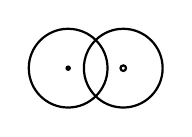
\begin{tikzpicture}[thick]

  \draw (2,0) circle (0.5cm);
  \draw (2.7,0) circle (0.5cm);
  \fill (2,0) circle (0.1em);
  \fill[white, draw=black] (2.7,0) circle (0.1em);

\end{tikzpicture}
\caption{Two atoms clashing, despite having different (though close) coordinates of their centres.}
\label{fig:atomsintersect}
\end{figure}

This makes a hash table unsuited for this purpose; two different coordinates would not map to the same atom. However, what if a region or volume could be hashed, rather than coordinates? Consider the 2-D drawing in figure \ref{fig:2dregionsmall}.

\begin{figure}[H]
\centering
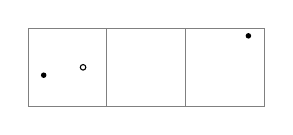
\begin{tikzpicture}

  \draw[step=1cm,gray,very thin] (0,0) grid (3,1);
  \fill (0.2,0.4) circle (0.1em);
  \fill[white, draw=black] (0.7,0.5) circle (0.1em);
  \fill (2.8,0.9) circle (0.1em);

\end{tikzpicture}
\caption{The rectangles represent areas, which can contain atoms. The dots represent the atom centres.}
\label{fig:2dregionsmall}
\end{figure}

Each rectangle is one area that could somehow be used as the key to the hash table, and each area can contain more than one atom whose coordinates fall inside it. The atoms from protein A are drawn in black and the atoms from protein B are drawn in white. In this example, the first area has one atom from protein A and one from protein B inside; i.e. a clash. The second area is empty, and the third has one atom from protein A.

An illustration of what a larger 2-D plane of one protein could look like is shown in figure \ref{fig:2dregionmap}. Each area could be enumerated in some way, for instance from the upper left corner. By assigning each area a predictable number, this ordinal can be used as the hash table key.

\begin{figure}[H]
\centering
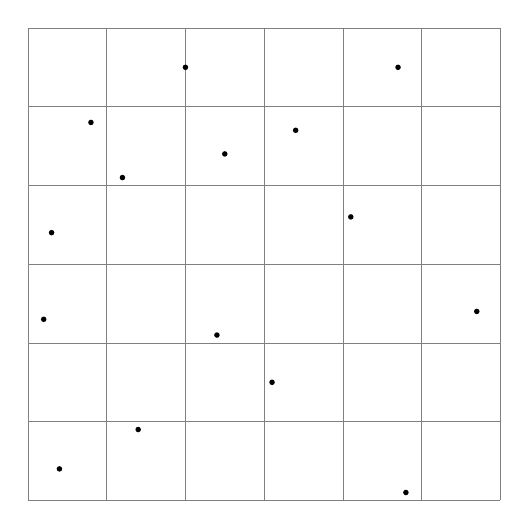
\begin{tikzpicture}

  \draw[step=1cm,gray,very thin] (0,0) grid (6,6);
  \fill (0.4,0.4) circle (0.1em);
  \fill (0.2,2.3) circle (0.1em);
  \fill (0.3,3.4) circle (0.1em);
  \fill (0.8,4.8) circle (0.1em);

  \fill (1.4,0.9) circle (0.1em);
  \fill (1.2,4.1) circle (0.1em);

  \fill (2.0,5.5) circle (0.1em);
  \fill (2.4,2.1) circle (0.1em);
  \fill (2.5,4.4) circle (0.1em);

  \fill (3.1,1.5) circle (0.1em);
  \fill (3.4,4.7) circle (0.1em);

  \fill (4.8,0.1) circle (0.1em);
  \fill (4.1,3.6) circle (0.1em);
  \fill (4.7,5.5) circle (0.1em);

  \fill (5.7,2.4) circle (0.1em);

\end{tikzpicture}
\caption{The spanned surface of the 2-D representation of some small molecule. The surface is divided into areas, which the atoms fall in.}
\label{fig:2dregionmap}
\end{figure}

The size of the areas' sides equals the diameter of the largest atom, in this case 4.0 Å. Notice that a clash can happen even though the atoms are not in the same area, however. Consider figure \ref{fig:clashindifferentareas}, where an atom from protein A is in the first area, and an atom from protein B is in the second. Given that the side of the area is 4.0 Å, the atoms are close enough to clash, despite being in different areas.

\begin{figure}[H]
\centering
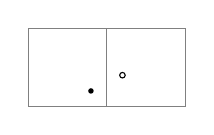
\begin{tikzpicture}

  \draw[step=1cm,gray,very thin] (0,0) grid (2,1);
  \fill (0.8,0.2) circle (0.1em);
  \fill[white, draw=black] (1.2,0.4) circle (0.1em);

\end{tikzpicture}
\caption{A clash between two atoms, despite them being in different areas.}
\label{fig:clashindifferentareas}
\end{figure}

In order to find all potential clashes for an atom that resides in some area, the areas adjacent to it will have to be searched as well. In the 2-D example, this would be $3 \cdot 3 = 9$ areas to look in. Figure \ref{fig:2dregionstosearch} illustrates the regions that have to be searched, if the atom to find clashes for is denoted by the small square.

\begin{figure}[H]
\centering
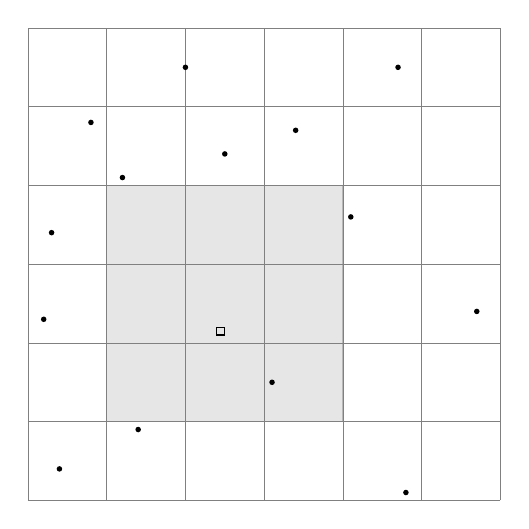
\begin{tikzpicture}

  \draw[fill=gray, opacity=0.2] (1,1) rectangle (4,4);
  \draw[step=1cm,gray,very thin] (0,0) grid (6,6);
  \fill (0.4,0.4) circle (0.1em);
  \fill (0.2,2.3) circle (0.1em);
  \fill (0.3,3.4) circle (0.1em);
  \fill (0.8,4.8) circle (0.1em);

  \fill (1.4,0.9) circle (0.1em);
  \fill (1.2,4.1) circle (0.1em);

  \fill (2.0,5.5) circle (0.1em);
  \draw (2.4,2.1) rectangle (2.5,2.2);
  \fill (2.5,4.4) circle (0.1em);

  \fill (3.1,1.5) circle (0.1em);
  \fill (3.4,4.7) circle (0.1em);

  \fill (4.8,0.1) circle (0.1em);
  \fill (4.1,3.6) circle (0.1em);
  \fill (4.7,5.5) circle (0.1em);

  \fill (5.7,2.4) circle (0.1em);

\end{tikzpicture}
\caption{The areas to search in, if the atom to find clashes for is located in the centre of the marked areas.}
\label{fig:2dregionstosearch}
\end{figure}

Of course, the proteins are in 3-D. Thus, a protein is divided into a space consisting of cubes with the sides being of length 4.0 Å. An illustration of the Crambin protein (1CRN) inside a space is shown in figure \ref{fig:3dspace}. Note that this is an illustration of the principle and the cubes are not to scale.

The space spanned by the atoms of protein A would be divided into cubes, and so would the atoms of protein B. Thus, similar to figure \ref{fig:2dregionstosearch}, for a given atom in one of the proteins, the cube that it falls inside will be calculated, and the $3 \cdot 3 \cdot 3 = 27$ adjacent cubes of the other protein will be looked in for a clash.

Thus, every atom of protein A will be assigned into the corresponding cube, and the cube-atom pair will be placed in a hash table. When searching for clashes, we can now go through every atom of protein B, find the 27 adjacent cubes of it and look them up in the hash table. While 27 lookups for an atom might seem costly, the number is constant no matter the size of the proteins. This solution is thus $O(n)$.

\begin{figure}[H]
\centering
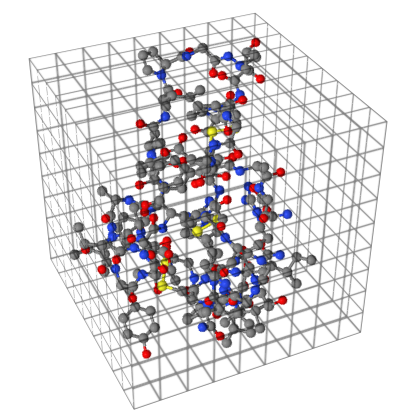
\includegraphics{res/molspace_big.png}
\caption{A protein inside a space of cubes.}
\label{fig:3dspace}
\end{figure}

The name Cubic Steric Overlap Detector comes from the described solution of detecting steric overlaps by dividing molecules into cubes.


\subsection*{Running}
The program can be run from the command-line or via a GUI. It has two ways of calculating the number of atom clashes: the ``hashing'' method and the ``brute force'' method. The former is the method that has been described in this document ($O(n)$), while the latter will compare every atom in protein A with every atom in protein B ($O(n^2)$). The brute force method is implemented as a reference, and not intended to be used in practice.

To run the program from the command-line, use\\
\texttt{java -jar csod.jar INPUT1.pdb INPUT2.pdb -METHOD OUTPUT.txt}\\
where \texttt{INPUT1.pdb} and \texttt{INPUT2.pdb} are the filenames of the *.pdb-files to read, \texttt{METHOD} is either \texttt{h} to use the ``hashing'' method or \texttt{b} to use the ``brute force'' method, and \texttt{OUTPUT.txt} is the name of the file to write the results to. If \texttt{OUTPUT.txt} is not given, the results will be written to 'output.txt'.


\section*{Overview of source code}
The ``cubes'' referred to previously, which the atoms are placed in, are called ``containers'' in the source code. This is motivated by the fact that the class has support for any number of dimensions, while cubes are of three dimensions.

\subsection*{\texttt{Main.java}}
The \texttt{main()} method will determine what to do based on the parameters sent to it. If no parameters are given, the GUI will start. The program can be run on the command line by giving the following parameters: \texttt{input\_filename1}, \texttt{input\_filename2}, \texttt{computing\_method}, \texttt{output\_filename}. The two first parameters is the path of the input files (previously referred to as protein A and B in this document). The \texttt{computing\_method} parameter specifies whether the ``hashing'' or ``brute force'' method should be used. The \texttt{output\_filename} parameter is optional; if given, it specifies the filename of the output data, if not given, the output will be written to the file ``output.txt''.

\subsection*{\texttt{Gui.java}}
This file only contains the code for the creation and layout of the GUI.

\subsection*{\texttt{Atom.java}}
Class for holding information about Atoms. The values are given from the *.pdb-files. Each Atom may also, optionally, hold an ArrayList of which containers in the Space that exist around it. These are the containers that are near the container that this Atom falls in. By pre-calculating these nearby containers, time can be saved during the comparison phase.

\subsection*{\texttt{HashEntry.java}}
This class acts as an entry for the HashMap. It contains an ArrayList of Pairs. The key of each Pair is an Integer, which corresponds to the container ordinal of the atoms; this is used to allow for hash collisions. The value of a Pair is the Atom, that is present in the container that the HashEntry corresponds to.

\subsection*{\texttt{Location.java}}
The Location class stores coordinates. Any number of dimensions can be handled. Internally, the coordinates are stored in \texttt{BigDecimal}s, which are less prone to rounding errors than doubles.

\subsection*{\texttt{Utils.java}}
This class contains miscellaneous utility methods. It contains code for reading *.pdb-files, performing the pre-calculations of setting up a Space and creating a HashMap, and also contains code for looping through the atoms of a *.pdb-file and looking for clashes in the atoms stored in the HashMap.

\subsection*{\texttt{Space.java}}
The Space class is used for obtaining the container ordinals of an atom. It can handle any number of dimensions. By giving the size of the sides of a container, as well as the minimum and maximum values of a molecule, it can calculate the container ordinal a location inside that space would fall it.

\end{document}
